% Author: Izaak Neutelings (March 2019)
\documentclass[border=3pt,tikz]{standalone}
\tikzset{>=latex} % for LaTeX arrow head

\tikzstyle{block}=[inner xsep=8,inner ysep=9,fill=red!60!black]
\tikzstyle{bin}=[inner xsep=8,inner ysep=3,fill=white,above=1]
\tikzstyle{arrow}=[->,thick,thick,blue!50!black,shorten <=1,shorten >=4]

\begin{document}



% RANDOM WALK
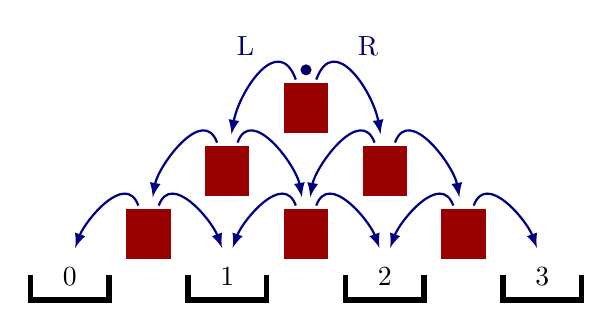
\begin{tikzpicture}
  \def\w{1}
  \def\h{.8}
  \def\bin{++ (\w/2,.3*\h) |-++ (-\w,-.4*\h) --++ (0,.4*\h)}
  
  \node[block] (S1-1) at (0,0) {};
  \node[block] (S2-1) at (-\w,-\h) {};
  \node[block] (S2-2) at (\w,-\h) {};
  \node[block] (S3-1) at (-2*\w,-2*\h) {};
  \node[block] (S3-2) at (0,-2*\h) {};
  \node[block] (S3-3) at (2*\w,-2*\h) {};
  \node[bin] (S4-1) at (-3*\w,-3*\h) {0};
  \node[bin] (S4-2) at (-\w,-3*\h) {1};
  \node[bin] (S4-3) at (\w,-3*\h) {2};
  \node[bin] (S4-4) at (3*\w,-3*\h) {3};
  %\coordinate (S4-1) at (-3*\w,-2.5*\h);
  %\coordinate (S4-2) at (-\w,-2.5*\h);
  %\coordinate (S4-3) at (\w,-2.5*\h);
  %\coordinate (S4-4) at (3*\w,-2.5*\h);
  
  \fill[blue!40!black] (90:0.6*\h) circle (2pt);
  
  % ROW 1
  \draw[arrow] (S1-1.110) to[out=110,in= 80,looseness=1.5] (S2-1.85)
    node[midway,above left=15,blue!40!black] {L};
  \draw[arrow] (S1-1. 70) to[out= 70,in=100,looseness=1.5] (S2-2.95)
    node[midway,above right=15,blue!40!black] {R};
  
  % ROW 2
  \draw[arrow] (S2-1.110) to[out=110,in= 80,looseness=1.2] (S3-1.85);
  \draw[arrow] (S2-1. 70) to[out= 70,in=100,looseness=1.2] (S3-2.95);
  \draw[arrow] (S2-2.110) to[out=110,in= 80,looseness=1.2] (S3-2.85);
  \draw[arrow] (S2-2. 70) to[out= 70,in=100,looseness=1.2] (S3-3.95);
  
  % ROW 3
  \draw[arrow] (S3-1.110) to[out=110,in= 70,looseness=1.2] (S4-1.85);
  \draw[arrow] (S3-1. 70) to[out= 70,in=110,looseness=1.2] (S4-2.95);
  \draw[arrow] (S3-2.110) to[out=110,in= 70,looseness=1.2] (S4-2.85);
  \draw[arrow] (S3-2. 70) to[out= 70,in=110,looseness=1.2] (S4-3.95);
  \draw[arrow] (S3-3.110) to[out=110,in= 70,looseness=1.2] (S4-3.85);
  \draw[arrow] (S3-3. 70) to[out= 70,in=110,looseness=1.2] (S4-4.95);
  
  % BIN
  \draw[line width=2] (S4-1.south) \bin;
  \draw[line width=2] (S4-2.south) \bin;
  \draw[line width=2] (S4-3.south) \bin;
  \draw[line width=2] (S4-4.south) \bin;
  
\end{tikzpicture}



\end{document}
